% Options for packages loaded elsewhere
\PassOptionsToPackage{unicode}{hyperref}
\PassOptionsToPackage{hyphens}{url}
%
\documentclass[
]{article}
\usepackage{amsmath,amssymb}
\usepackage{lmodern}
\usepackage{iftex}
\ifPDFTeX
  \usepackage[T1]{fontenc}
  \usepackage[utf8]{inputenc}
  \usepackage{textcomp} % provide euro and other symbols
\else % if luatex or xetex
  \usepackage{unicode-math}
  \defaultfontfeatures{Scale=MatchLowercase}
  \defaultfontfeatures[\rmfamily]{Ligatures=TeX,Scale=1}
\fi
% Use upquote if available, for straight quotes in verbatim environments
\IfFileExists{upquote.sty}{\usepackage{upquote}}{}
\IfFileExists{microtype.sty}{% use microtype if available
  \usepackage[]{microtype}
  \UseMicrotypeSet[protrusion]{basicmath} % disable protrusion for tt fonts
}{}
\makeatletter
\@ifundefined{KOMAClassName}{% if non-KOMA class
  \IfFileExists{parskip.sty}{%
    \usepackage{parskip}
  }{% else
    \setlength{\parindent}{0pt}
    \setlength{\parskip}{6pt plus 2pt minus 1pt}}
}{% if KOMA class
  \KOMAoptions{parskip=half}}
\makeatother
\usepackage{xcolor}
\IfFileExists{xurl.sty}{\usepackage{xurl}}{} % add URL line breaks if available
\IfFileExists{bookmark.sty}{\usepackage{bookmark}}{\usepackage{hyperref}}
\hypersetup{
  pdftitle={Assignment 2: Interpreting Quantitative Findings},
  hidelinks,
  pdfcreator={LaTeX via pandoc}}
\urlstyle{same} % disable monospaced font for URLs
\usepackage[margin=1in]{geometry}
\usepackage{graphicx}
\makeatletter
\def\maxwidth{\ifdim\Gin@nat@width>\linewidth\linewidth\else\Gin@nat@width\fi}
\def\maxheight{\ifdim\Gin@nat@height>\textheight\textheight\else\Gin@nat@height\fi}
\makeatother
% Scale images if necessary, so that they will not overflow the page
% margins by default, and it is still possible to overwrite the defaults
% using explicit options in \includegraphics[width, height, ...]{}
\setkeys{Gin}{width=\maxwidth,height=\maxheight,keepaspectratio}
% Set default figure placement to htbp
\makeatletter
\def\fps@figure{htbp}
\makeatother
\setlength{\emergencystretch}{3em} % prevent overfull lines
\providecommand{\tightlist}{%
  \setlength{\itemsep}{0pt}\setlength{\parskip}{0pt}}
\setcounter{secnumdepth}{5}
\newlength{\cslhangindent}
\setlength{\cslhangindent}{1.5em}
\newlength{\csllabelwidth}
\setlength{\csllabelwidth}{3em}
\newlength{\cslentryspacingunit} % times entry-spacing
\setlength{\cslentryspacingunit}{\parskip}
\newenvironment{CSLReferences}[2] % #1 hanging-ident, #2 entry spacing
 {% don't indent paragraphs
  \setlength{\parindent}{0pt}
  % turn on hanging indent if param 1 is 1
  \ifodd #1
  \let\oldpar\par
  \def\par{\hangindent=\cslhangindent\oldpar}
  \fi
  % set entry spacing
  \setlength{\parskip}{#2\cslentryspacingunit}
 }%
 {}
\usepackage{calc}
\newcommand{\CSLBlock}[1]{#1\hfill\break}
\newcommand{\CSLLeftMargin}[1]{\parbox[t]{\csllabelwidth}{#1}}
\newcommand{\CSLRightInline}[1]{\parbox[t]{\linewidth - \csllabelwidth}{#1}\break}
\newcommand{\CSLIndent}[1]{\hspace{\cslhangindent}#1}
\usepackage{amsmath}
\usepackage{booktabs}
\usepackage{lastpage}
\usepackage{fancyhdr}
\pagestyle{fancy}
\fancyhead{}
\renewcommand{\headrulewidth}{0pt}
\fancyfoot[CO,CE]{Page \thepage\ of \pageref{LastPage}}
\usepackage{floatrow}
\floatsetup[figure]{capposition=top}
\floatsetup[table]{capposition=top}
\usepackage{setspace}
\usepackage{booktabs}
\usepackage{longtable}
\usepackage{array}
\usepackage{multirow}
\usepackage{wrapfig}
\usepackage{float}
\usepackage{colortbl}
\usepackage{pdflscape}
\usepackage{tabu}
\usepackage{threeparttable}
\usepackage{threeparttablex}
\usepackage[normalem]{ulem}
\usepackage{makecell}
\usepackage{xcolor}
\ifLuaTeX
  \usepackage{selnolig}  % disable illegal ligatures
\fi

\title{Assignment 2: Interpreting Quantitative Findings}
\usepackage{etoolbox}
\makeatletter
\providecommand{\subtitle}[1]{% add subtitle to \maketitle
  \apptocmd{\@title}{\par {\large #1 \par}}{}{}
}
\makeatother
\subtitle{\hfill\break
University of Glasgow\\
\strut \\
Student ID: 2819052\\
Course: Quantitative Methods in the Social Sciences\\
Number of words: 2747\\}
\author{}
\date{\vspace{-2.5em}}

\begin{document}
\maketitle

\pagebreak

\setcounter{tocdepth}{2}
\tableofcontents

\pagebreak

\hypertarget{introduction}{%
\section{Introduction}\label{introduction}}

\doublespacing 

In 1998, the Good Friday/Belfast Agreement was signed and later
validated by the voters, and this agreement marked a new era of hope
towards peace, equality, and inclusion in Northern Ireland
(\protect\hyperlink{ref-galligan2013gender}{Galligan 2013}). The main
focus on the agreement and referendum was obviously to stop the violent
conflict and seek peace, but a part of the agreement also emphasized an
equality agenda (\protect\hyperlink{ref-Hayward2021}{Hayward 2021}).
Thus, the agreement also marked the first Northern Irish formal
recognition of women's rights to political inclusion
(\protect\hyperlink{ref-galligan2013gender}{Galligan 2013}). However, a
formal recognition does not necessarily imply that gender equality
trickles down into societal norms and practices. Therefore, this report
examines the contemporary state of women's equality in Northern Ireland.

Perhaps, the most central concept within gender equality is the
\emph{gender pay gap}. Disparities in income is an important indicator
for gender equality, because it has social, economic, and physiological
consequences (\protect\hyperlink{ref-bishu2017gender}{Bishu and Alkadry
2017}). Research on this area have identified several factors that seems
to influence a gender pay gap. One such factor can be inequality in
access to workplace authority, where women are denied manager or
supervisor position although there were equally qualified
(\protect\hyperlink{ref-bishu2017gender}{Bishu and Alkadry 2017}). Other
factors can be discrimination in hiring or promotion processes, but also
lack of gender representation can avoid minorities to even apply for a
job or promotion (\protect\hyperlink{ref-bishu2017gender}{Bishu and
Alkadry 2017}).

In order to examine the current gender equality in Northern Ireland, we
therefore focus on the gender pay gap in Northern Ireland. We ask the
following research question: \emph{Does gender affect income in
contemporary Northern Ireland?} We employ a deductive approach, where we
first formulate a hypothesis and subsequently examine it empirically
(\protect\hyperlink{ref-bryman2016social}{Bryman 2016, 33}). Therefore,
our analysis consider the following null hypothesis (H\textsubscript{0})
and alternative hypothesis (H\textsubscript{A}):

\begin{itemize}
\tightlist
\item
  H\textsubscript{0}: Being a woman or man does not affect your income.
\item
  H\textsubscript{A}: Being a woman rather than a man affects a lower
  income.
\end{itemize}

The causal relationship that we examine is thus a negative relationship.
Although, we call this relationship causal, it is important to clarify
that I do not imply that there is anything biological or deterministic
that reduce women's income in general. Rather, the causal link is
interpreted as a result of the societal discriminatory practices
explained in the previous paragraph. To make a convincing inquiry of
this causal relationship, we must also control for a number of other
factors related to income and gender. This is important to make sure
that our analysis do not simply show a spurious correlation as it could
in fact be another factor that influences both gender and income. These
control variables are introduced in
\protect\hyperlink{data-and-method}{Data and Method}.

\pagebreak

\hypertarget{data-and-method}{%
\section{Data and Method}\label{data-and-method}}

The research design of this analysis is a cross-sectional design
(\protect\hyperlink{ref-bryman2016social}{Bryman 2016, 53}). This means
that the data for analysis is collected at a single point in time and
consists of a sample of respondents from which we seek to infer to a
general population of Northern Ireland
(\protect\hyperlink{ref-field2012discovering}{Field, Miles, and Field
2012, 36}). This section describes this sample and how the data was
collected, and then subsequently the operationalized variables to
examine our research hypothesis are described.

\hypertarget{sample-and-data-collection}{%
\subsection{Sample and Data
Collection}\label{sample-and-data-collection}}

Our sample of analysis consists of data from the Northern Ireland Life
and Times Survey (NILT). The data have been collected every year since
1998, but this analysis uses the survey from 2012
(\protect\hyperlink{ref-ark_2012}{ARK 2012}). The respondents for the
NILT survey was chosen from a systematic random sample of addresses.
From this sample of 2126 addresses, 1204 questionnaires were fully
completed using partly face-to-face- and self-completion questionnaires
(\protect\hyperlink{ref-ark_2012}{ARK 2012}). Our sample of analysis is
further reduced as not all respondents have answered our variables of
interest, and we are therefore not able to include those respondents in
our analysis. In the tables below, we present descriptive statistics for
our variables of interest in both the full NILT sample and our sample of
analysis. The first tables shows the categorical variables, where a
frequency distribution are shown
(\protect\hyperlink{ref-fogarty2018quantitative}{Fogarty 2018, 88}). The
second table shows the numerical variables, where we have calculated the
mean and standard deviation
(\protect\hyperlink{ref-fogarty2018quantitative}{Fogarty 2018, 95}). For
a full visualization of all variables included in the analysis, see
\protect\hyperlink{appendix}{Appendix}.

\begin{table}[H]

\caption{\label{tab:unnamed-chunk-1}Descriptive Statistics for Cleaned and Full Sample (Categorical Variables)}
\centering
\begin{tabular}[t]{llllll}
\toprule
\multicolumn{1}{c}{ } & \multicolumn{2}{c}{Cleaned Sample} & \multicolumn{2}{c}{Full Sample} & \multicolumn{1}{c}{ } \\
\cmidrule(l{3pt}r{3pt}){2-3} \cmidrule(l{3pt}r{3pt}){4-5}
Variable & N & Percent & N & Percent & Test\\
\midrule
Gender & 675 &  & 1204 &  & X2=1.022\\
... Male & 284 & 42.1\% & 537 & 44.6\% & \\
... Female & 391 & 57.9\% & 667 & 55.4\% & \\
Religion & 675 &  & 1168 &  & X2=0.849\\
... Catholic & 277 & 41\% & 491 & 42\% & \\
\addlinespace
... Protestant & 283 & 41.9\% & 497 & 42.6\% & \\
... No religion & 115 & 17\% & 180 & 15.4\% & \\
Sexual Orientation & 675 &  & 1191 &  & X2=3.039\\
... I am heterosexual or straight & 657 & 97.3\% & 1173 & 98.5\% & \\
... I am gay or lesbian (homosexual) & 14 & 2.1\% & 14 & 1.2\% & \\
\addlinespace
... I am bi-sexual & 2 & 0.3\% & 2 & 0.2\% & \\
... Other & 2 & 0.3\% & 2 & 0.2\% & \\
Constitutional View & 675 &  & 1183 &  & X2=0.347\\
... Unionist & 199 & 29.5\% & 348 & 29.4\% & \\
... Nationalist & 138 & 20.4\% & 255 & 21.6\% & \\
\addlinespace
... Neither & 338 & 50.1\% & 580 & 49\% & \\
Trade union membership & 675 &  & 1179 &  & X2=9.162***\\
... No & 374 & 55.4\% & 739 & 62.7\% & \\
... Yes & 301 & 44.6\% & 440 & 37.3\% & \\
Supervisor: No & 675 &  & 883 &  & X2=0.143\\
\addlinespace
... No & 464 & 68.7\% & 616 & 69.8\% & \\
... Yes & 211 & 31.3\% & 267 & 30.2\% & \\
\bottomrule
\multicolumn{6}{l}{\rule{0pt}{1em}\textit{Note: }}\\
\multicolumn{6}{l}{\rule{0pt}{1em}Statistical significance markers: * p<0.1; ** p<0.05; *** p<0.01}\\
\end{tabular}
\end{table}

\begin{table}[H]

\caption{\label{tab:unnamed-chunk-1}Descriptive Statistics for Cleaned and Full Sample (Numerical Variables)}
\centering
\begin{tabular}[t]{llllllll}
\toprule
\multicolumn{1}{c}{ } & \multicolumn{3}{c}{Cleaned Sample} & \multicolumn{3}{c}{Full Sample} & \multicolumn{1}{c}{ } \\
\cmidrule(l{3pt}r{3pt}){2-4} \cmidrule(l{3pt}r{3pt}){5-7}
Variable & N & Mean & SD & N & Mean & SD & Test\\
\midrule
Annual Personal Income (GBP) & 675 & 16892.089 & 13447.704 & 897 & 16394.582 & 13465.9 & F=0.526\\
Age & 675 & 46.763 & 17.117 & 1201 & 49.615 & 18.53 & F=10.81***\\
\bottomrule
\multicolumn{8}{l}{\rule{0pt}{1em}\textit{Note: }}\\
\multicolumn{8}{l}{\rule{0pt}{1em}Statistical significance markers: * p<0.1; ** p<0.05; *** p<0.01}\\
\end{tabular}
\end{table}

As the table shows, our sample is significantly reduced by removing
missing values - from 1204 observations to 675 observations. In the
table with categorical variables, we conduct a Chi-squared test to check
if there is independence between the samples or not, i.e.~whether the
frequency distribution is significantly different
(\protect\hyperlink{ref-fogarty2018quantitative}{Fogarty 2018, 176}).
For the numerical variables, we conduct an Analysis of Variances (ANOVA)
to test whether the means in the two samples are significantly different
(\protect\hyperlink{ref-field2012discovering}{Field, Miles, and Field
2012, 399ff}). For the categorical variables, we see that for the test
of trade union membership, the test value is 9.162, which is
significantly different from 0 (with a p-value less than 0.01). This
indicates that the frequency distribution in our sample is significantly
different from the full NILT sample. There is a larger share (44.6 \%)
of members of a trade union after removing missing values compared to
only 37.3 \% in the full NILT sample. Similarly, we see from the ANOVA
that the test value (F) for age is significantly different from 0 (with
a p-value less than 0.01) meaning that our sample is different from the
full NILT sample in the age distribution. We can see that the mean age
is only around 46 years compared to 49 years in the full NILT sample.
These two findings are important to bear in mind, when we interpret our
final conclusion as both age and trade union membership might be related
to our dependent variable, income.

The systematic random sampling strategy in the NILT survey is an
approach to make the sample representative of our population - in our
case all inhabitants of Northern Ireland. It could be relevant to
examine the demographic distribution in our sample against the general
population of Northern Ireland, but unfortunately that is beyond the
scope of this report.

\hypertarget{dependent-and-independent-variables}{%
\subsection{Dependent and Independent
Variables}\label{dependent-and-independent-variables}}

In order to examine the research question empirically, we operationalize
the concepts included in our hypothesis as measurable variables. As the
questionnaire was formulated beforehand in the NILT 2012 survey, the
data is a secondary source, as we have to find the questions that can
represent our theoretical concepts.

The dependent variable or outcome that we want to explain in this
analysis is income. Although income in itself is more concrete concept
compared to other theoretical concepts in social science (such as
e.g.~``solidarity''), it can still be measured in many different ways.
In this analysis, we measure income by the question: \emph{What is your
personal income before tax and national insurance contributions? (£ per
year)}. It is thus a numeric, more specifically a ratio scale with a
value of absolute zero - although it is quite uncommon to have a
personal income of zero
(\protect\hyperlink{ref-fogarty2018quantitative}{Fogarty 2018, 56}).

The independent variable or explanatory variable of our analysis is
gender. Gender is a much more complex concept, and there is a large
discussion about the distinction between gender and sex, and the
biological and cultural components of these
(\protect\hyperlink{ref-unger1993sex}{Unger and Crawford 1993}).
Quantitative research have mostly been dominated by gender being
measured as a binary division between male and female. Likewise, we are
also limited to such a measurement of gender in the NILT 2012 survey. In
this analysis, we therefore measure gender by a nominal, binary variable
of either ``male'' or ``female''.

To consider the distribution of our dependent and independent variable,
see the following scatter plot of income and gender. In the scatter
plot, we also show the mean and median income for each group of gender
by the solid and dashed lines.

\begin{figure}[H]

{\centering 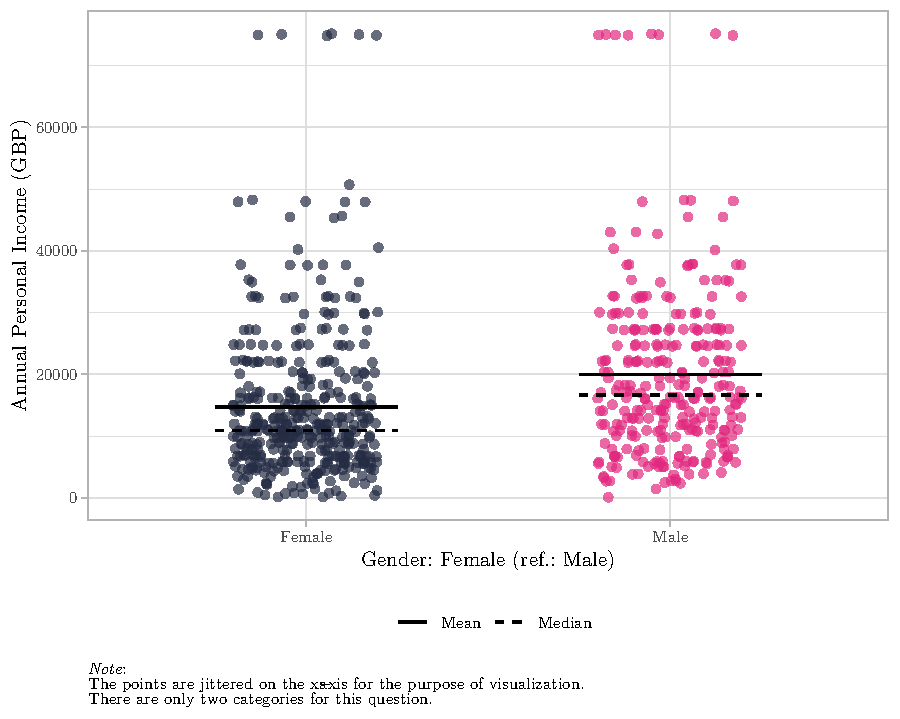
\includegraphics[width=0.8\linewidth]{paper_files/figure-latex/unnamed-chunk-2-1} 

}

\caption{Scatterplot of Income and Gender}\label{fig:unnamed-chunk-2}
\end{figure}

There are several insights from this visualization. The vertical
differences between the descriptive statistics, mean and median
signifies that there is a general income difference between males and
females, and that females in average have lower incomes than men.
Initially, this suggests an acceptance of our alternative research
hypothesis, but we will wait with any conclusion till the analysis,
where we also control for other related factors. Another interesting
insight is that the distribution of income seems to be slightly skewed.
For both males and females, there are some respondents with a very high
income compared to most other respondents. This can also noticed as
there is a difference between the mean and the median for both groups.
These respondents have such extreme high incomes that they might be
outliers compared to the general trend, and we need to be aware of that
in our analysis (\protect\hyperlink{ref-fogarty2018quantitative}{Fogarty
2018, 221--22}).

\hypertarget{control-variables}{%
\subsection{Control Variables}\label{control-variables}}

Theoretically, there are other characteristics than gender than might
affect your income. Firstly, there are characteristics related to your
work that might affect a higher salary that is not rooted in
discriminatory practices. To make sure that an effect of gender is not
just a result these factor, we find it relevant to include trade union
membership and whether or not someone has a formal responsibility for
supervising the work of other employees
(\protect\hyperlink{ref-ark_2012}{ARK 2012}). Moreover, there can also
be other characteristics that affect a lower income based in
discriminatory practices that is not rooted upon one's gender.
Therefore, we also include religion, sexual orientation, constitutional
view, and age into our analysis as control variables.

\hypertarget{method-of-analysis}{%
\subsection{Method of Analysis}\label{method-of-analysis}}

To fully examine the relationship between our dependent and independent
variable, we employ a multiple linear regression estimated with OLS
(\protect\hyperlink{ref-fogarty2018quantitative}{Fogarty 2018, 192ff}).
Thus, we are also able to include the control variables to make the
acceptance or decline of our hypothesis more convincing. The formula of
the regression of our analysis is thus: \begin{align*}
\hat income = \beta_0 + \beta_1*gender + \beta_2 * religion + \beta_3 * Sexual Orientation \\ + \beta_4 * Constitutional View +  \beta_5*Trade Union Membership + \beta_6*Supervisor + \varepsilon
\end{align*}

where the main parameter of interest is \(\beta_1\) for gender.

\pagebreak

\hypertarget{results-and-discussion}{%
\section{Results and discussion}\label{results-and-discussion}}

This report examines the question of whether gender affect income in
contemporary Northern Ireland. As described in the
\protect\hyperlink{introduction}{Introduction}, the analysis therefore
seeks to accept whether the null hypothesis or the alternative
hypothesis - that being a woman rather than a man affects a lower
income. As described in the \protect\hyperlink{data-and-method}{Data and
Method} section, our analysis consists of survey data, where our main
variables are gender and personal income. To examine our hypothesis, the
following table shows the results of two regressions. First, our model
is shown as a bivariate regression excluding our control variables, and
secondly our full model is shown including our control variables.

\begin{table}[H] \centering 
  \caption{Regression results} 
  \label{} 
\small 
\begin{tabular}{@{\hspace{5pt}}l@{\hspace{5pt}}cc} 
\toprule 
 & \multicolumn{2}{c}{Dependent Variable} \\ 
\cmidrule(rr){2-3} 
 & \multicolumn{2}{c}{Annual Personal Income (GBP)} \\ 
 \cmidrule(rr){2-3}
 & Model excl. controls & Model incl. controls \\ 
\midrule  
\\[-2.1ex] Gender: Female (ref.: Male) & $-$5,234.993$^{***}$ & $-$5,068.737$^{***}$ \\ 
  & (1,029.652) & (994.748) \\ 
 \addlinespace 
 Religion: Protestant (ref.: Catholic) &  & 465.188 \\ 
  &  & (1,458.367) \\ 
 \addlinespace 
 Religion: No religion &  & 895.169 \\ 
  &  & (1,533.323) \\ 
 \addlinespace 
 Sexual Orientation: Homosexual (ref.: Heterosexual) &  & $-$6,247.777$^{*}$ \\ 
  &  & (3,437.048) \\ 
 \addlinespace 
 Sexual Orientation: bi-sexual &  & $-$2,826.980 \\ 
  &  & (8,698.806) \\ 
 \addlinespace 
 Sexual Orientation: Other &  & 1,323.336 \\ 
  &  & (8,737.282) \\ 
 \addlinespace 
 Constitutional View: Nationalist (ref.: Unionist) &  & 1,788.873 \\ 
  &  & (1,898.294) \\ 
 \addlinespace 
 Constitutional view: Neither &  & 1,438.036 \\ 
  &  & (1,350.423) \\ 
 \addlinespace 
 Trade union membership: Yes (ref.: No) &  & 5,277.978$^{***}$ \\ 
  &  & (977.008) \\ 
 \addlinespace 
 Supervisor: Yes (ref.: No) &  & 8,648.320$^{***}$ \\ 
  &  & (1,037.559) \\ 
 \addlinespace 
 Age &  & $-$84.369$^{***}$ \\ 
  &  & (29.430) \\ 
 \addlinespace 
 Constant & 19,924.510$^{***}$ & 17,417.240$^{***}$ \\ 
  & (783.659) & (2,223.337) \\ 
 \addlinespace 
\midrule  
Observations & 675 & 675 \\ 
R$^{2}$ & 0.037 & 0.183 \\ 
Adjusted R$^{2}$ & 0.036 & 0.170 \\ 
Residual Std. Error & 13,206.460 (df = 673) & 12,252.840 (df = 663) \\ 
F Statistic & 25.849$^{***}$ (df = 1; 673) & 13.533$^{***}$ (df = 11; 663) \\ 
\bottomrule 
\textit{Note:}  & \multicolumn{2}{r}{$^{*}$p$<$0.1; $^{**}$p$<$0.05; $^{***}$p$<$0.01} \\ 
\end{tabular} 
\end{table}

The primary finding from the regression results is that the variable
gender have an significant effect on income. We see that the p-value is
less than 0.01. This indicates that there is indeed a significant
difference between the income of men and women. However, a significant
p-value does not by itself means that the difference is important or
meaningful - we also need to interpret the effect size
(\protect\hyperlink{ref-field2012discovering}{Field, Miles, and Field
2012, 57}). If we take a look at the effect size (\(\beta_1\)), it has a
value of approx -5,068. Thus according to the model, women in average
earns 5,068 pounds a year less than men. That seems quite substantial as
the average income in our sample is 16,892 pounds a year (See Table 2).
Based on our analysis, we therefore accept our alternative hypothesis -
that being a woman rather than a man has a significant negative effect
in your income.

In the model, where we include our control variables, we see that trade
union membership and being a supervisor has a significant positive
effect on income, whereas age and to some extent also having a
homosexual orientation rather than a heterosexual orientation have a
significant negative effect on income. However, the effect of gender is
independent of religion, sexual orientation, constitutional view, trade
union membership, being a supervisor, and age, as including these
control variables into the regression does not render the effect of
gender on income insignificant. If we compare the model with and without
control variables, we see that both \(R^2\) and adjusted \(R^2\) is
increased with indicates that including the control variables does
indeed yield a better fit of data.

In this way, our empirical findings support the argument that there is
still a gender pay gap in Northern Ireland. Our finding that the gap
between men and women is independent of being a supervisor or not is
particularly interesting. It suggests that the income gap between men
and women exists for both, and the gender pay gap cannot only be
explained by men more often being in leadership positions. In the
following visualization, this finding can be seen clearly.

\begin{figure}[H]

{\centering 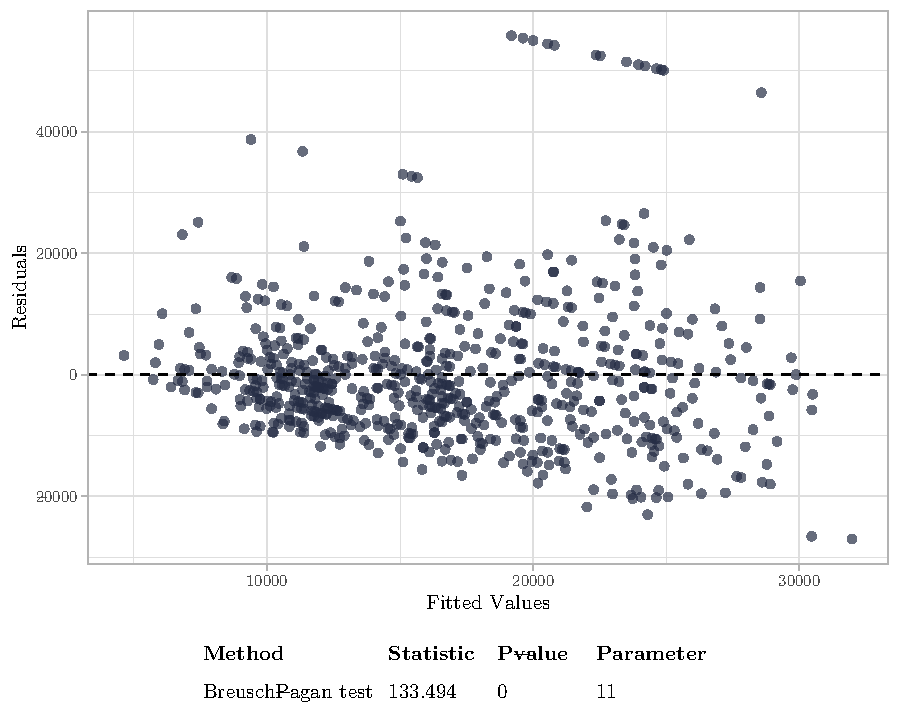
\includegraphics[width=0.8\linewidth]{paper_files/figure-latex/unnamed-chunk-4-1} 

}

\caption{Scatterplot of Income, Gender, and Supervisor}\label{fig:unnamed-chunk-4}
\end{figure}

In the visualization, there is also shown two linear regression of
gender on income, and we see that both slopes indicate a negative
correlation - although the intercepts differ.

Before concluding on our empirical results, it is also important to
consider how reliable our regression model is. One relevant concern of
our analysis is the influence of outliers, i.e.~very influential data
points (\protect\hyperlink{ref-fogarty2018quantitative}{Fogarty 2018,
221--22}; \protect\hyperlink{ref-field2012discovering}{Field, Miles, and
Field 2012, 190}). As identified in the {[}Data and Methods{]} section,
the dependent variables seems to have a data points with incomes that
are very much higher. Most respondents have an income around 17,000
pounds a year, while a few respondents have a yearly income around more
than 60,000 pounds. It is beyond the scope of this report to examine
whether these data points are in fact significant outliers, but it is
important to notice when interpreting the results.

Another concern to our model is heteroscedasticity, i.e.~whether there
is not a constant variance of residuals on the levels of the dependent
variable, income (\protect\hyperlink{ref-field2012discovering}{Field,
Miles, and Field 2012, 272}). In the plot below, we visualize the fitted
values with the residuals to see if the variances is constant along the
x-axis. Below the plot is also shown the results of a Breusch-Pagan test
to more formally test for heteroscedasticity
(\protect\hyperlink{ref-fogarty2018quantitative}{Fogarty 2018, 228}).

\begin{figure}[H]

{\centering 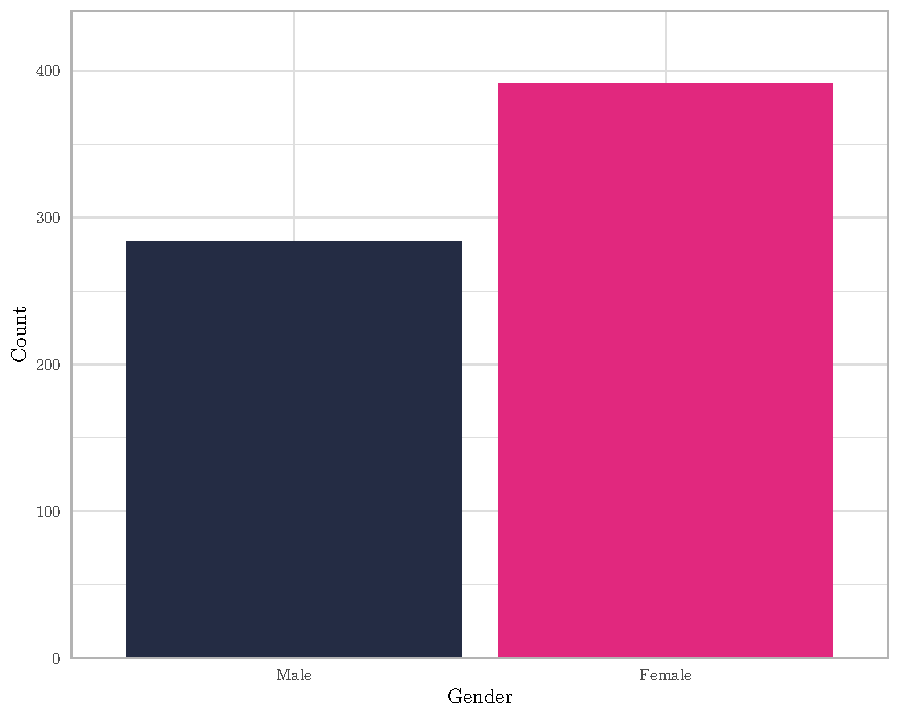
\includegraphics[width=0.8\linewidth]{paper_files/figure-latex/unnamed-chunk-5-1} 

}

\caption{Scatterplot of Fitted Values and Residuals}\label{fig:unnamed-chunk-5}
\end{figure}

Unfortunately, the plot shows that the variance seem to increase for
higher values of our dependent variables, income, and the Breusch-Pagan
test also suggests that there is heteroscedasticity as the p-value is
lower than 0.001. One solution to this problem could be to re-estimate
our regression model with robust standard errors, but this has not been
possible within the scope of this report
(\protect\hyperlink{ref-fogarty2018quantitative}{Fogarty 2018, 229}).

\pagebreak

\hypertarget{conclusion}{%
\section{Conclusion}\label{conclusion}}

Based on Northern Ireland as a historical case, this report has examined
the gender pay gap in the contemporary society of Northern Ireland.
Previous research has suggested that inclusion of statements about
gender equality does not necessarily trickle down into the everyday
practices, and this report therefore sought to examine this causal
relation empirically. The analysis tackles the research question:
\emph{Does gender affect income in contemporary Northern Ireland?} with
the alternative hypothesis that being a woman rather than a man affects
a lower income.

Using a survey-based research design, we employed a multivariate linear
regression analysis to answer this question. Our analysis showed that
there is indeed a gender pay gap in contemporary Northern Ireland. We
found that being a woman compared to a man resulted in average of an
approx. 5000 pounds lower yearly income - independent of factors such as
trade union membership, being a supervisor, age and more. Here, it is
particularly interesting that the effect of gender on income is
independent of having supervision, because it suggests that the gender
inequality exists across having a leadership position or not. Thus, our
analysis supports the arguments that gender affects income rooted in
discriminatory practices as theory suggests.

However, there are also limitations to our study that it is important to
take into concern. Firstly, there might be a few influential data points
- so-called outliers - that drives the effect to be larger than the
general trend. Secondly, we identified heteroscedasticity in our model,
and especially large incomes seems to have larger residuals. These are
primarily limitations of the reliability of the study, since it concerns
the model and methodological choices
(\protect\hyperlink{ref-bryman2016social}{Bryman 2016, 41}). If these
results can be reproduced with a model with robust standard errors or
after a check for outliers, it would increase the reliability of our
findings. Another point of discussion is the validity of our findings,
and here there is mostly the question of external validity as our sample
is reduced significantly during the data-cleaning process
(\protect\hyperlink{ref-bryman2016social}{Bryman 2016, 41--42}). A
further improvement here could have been to directly analyze if the
respondents in our data are representative compared to the general
population of Northern Ireland.

\pagebreak

\hypertarget{references}{%
\section{References}\label{references}}

\hypertarget{refs}{}
\begin{CSLReferences}{1}{0}
\leavevmode\vadjust pre{\hypertarget{ref-ark_2012}{}}%
ARK. 2012. \emph{2012 Northern Ireland Life \&Amp; Times Survey:
Technical Notes}. ARK. \url{https://www.ark.ac.uk/nilt/2012/tech12.pdf}.

\leavevmode\vadjust pre{\hypertarget{ref-bishu2017gender}{}}%
Bishu, Sebawit G., and Mohamad G. Alkadry. 2017. {``A Systematic Review
of the Gender Pay Gap and Factors That Predict It.''}
\emph{Administration \& Society} 49 (1): 65--104.
\url{https://doi.org/10.1177/0095399716636928}.

\leavevmode\vadjust pre{\hypertarget{ref-bryman2016social}{}}%
Bryman, A. 2016. \emph{Social Research Methods}. Oxford University
Press. \url{https://books.google.co.uk/books?id=N2zQCgAAQBAJ}.

\leavevmode\vadjust pre{\hypertarget{ref-field2012discovering}{}}%
Field, A., J. Miles, and Z. Field. 2012. \emph{Discovering Statistics
Using r}. SAGE Publications.
\url{https://books.google.co.uk/books?id=wd2K2zC3swIC}.

\leavevmode\vadjust pre{\hypertarget{ref-fogarty2018quantitative}{}}%
Fogarty, B. J. 2018. \emph{Quantitative Social Science Data with r: An
Introduction}. Core Textbook. SAGE Publications.
\url{https://books.google.co.uk/books?id=jwJ6DwAAQBAJ}.

\leavevmode\vadjust pre{\hypertarget{ref-galligan2013gender}{}}%
Galligan, Yvonne. 2013. {``Gender and Politics in Northern Ireland: The
Representation Gap Revisited.''} \emph{Irish Political Studies} 28 (3):
413--33.

\leavevmode\vadjust pre{\hypertarget{ref-Hayward2021}{}}%
Hayward, Katy. 2021. {``The 1998 Good Friday (Belfast) Agreement
Referendums in Northern Ireland and the Republic of Ireland.''} In
\emph{The Palgrave Handbook of European Referendums}, edited by Julie
Smith, 247--65. Cham: Springer International Publishing.
\url{https://doi.org/10.1007/978-3-030-55803-1_12}.

\leavevmode\vadjust pre{\hypertarget{ref-unger1993sex}{}}%
Unger, Rhoda K, and Mary Crawford. 1993. {``Sex and Gender---the
Troubled Relationship Between Terms and Concepts.''} \emph{Psychological
Science} 4 (2): 122--24.

\end{CSLReferences}

\pagebreak

\hypertarget{appendix}{%
\section{Appendix}\label{appendix}}

\begin{figure}[H]

{\centering 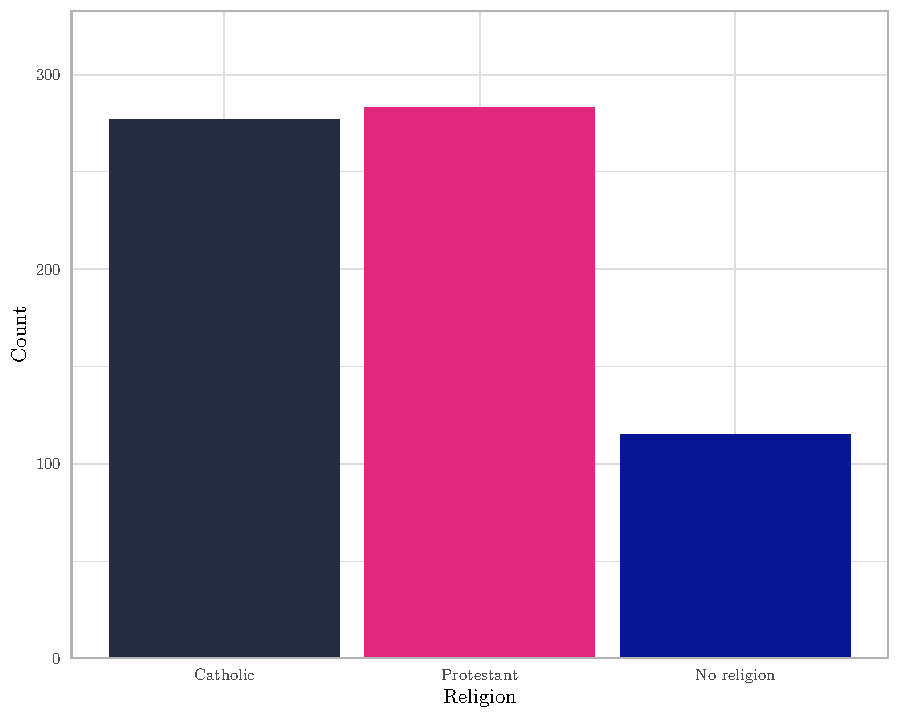
\includegraphics[width=0.8\linewidth]{paper_files/figure-latex/unnamed-chunk-6-1} 

}

\caption{Bar plot of Gender}\label{fig:unnamed-chunk-6}
\end{figure}

\begin{figure}[H]

{\centering 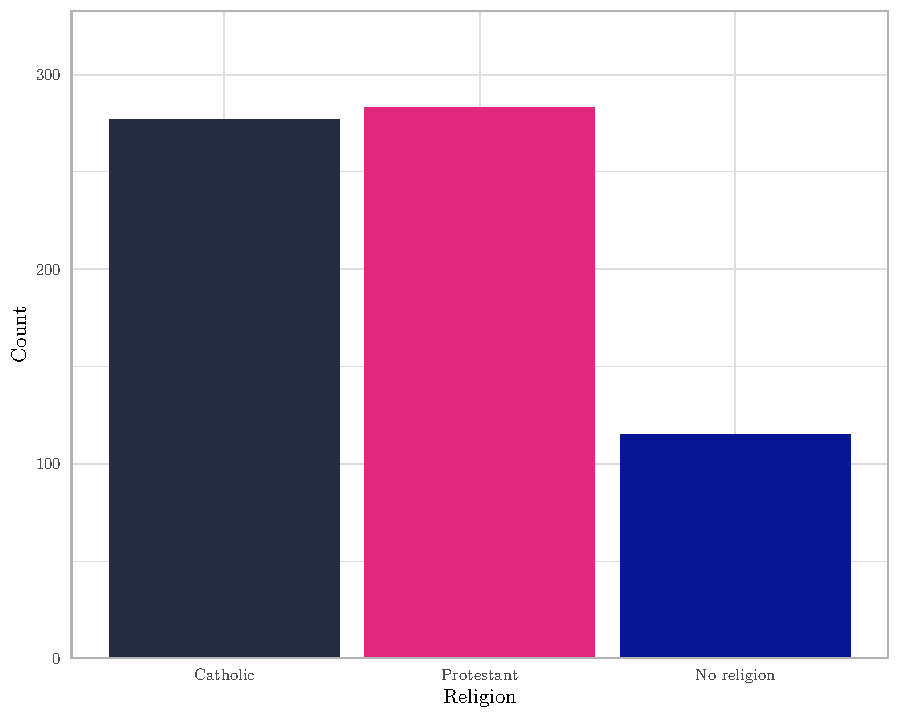
\includegraphics[width=0.8\linewidth]{paper_files/figure-latex/unnamed-chunk-7-1} 

}

\caption{Bar plot of Religion}\label{fig:unnamed-chunk-7}
\end{figure}

\begin{figure}[H]

{\centering 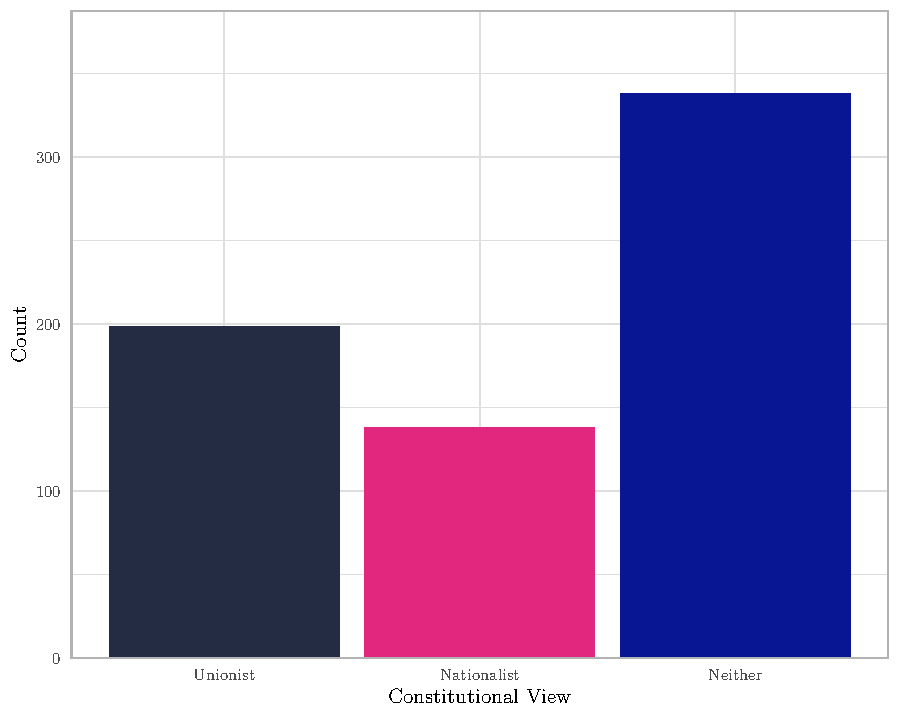
\includegraphics[width=0.8\linewidth]{paper_files/figure-latex/unnamed-chunk-8-1} 

}

\caption{Bar plot of Sexual Orientation}\label{fig:unnamed-chunk-8}
\end{figure}

\begin{figure}[H]

{\centering 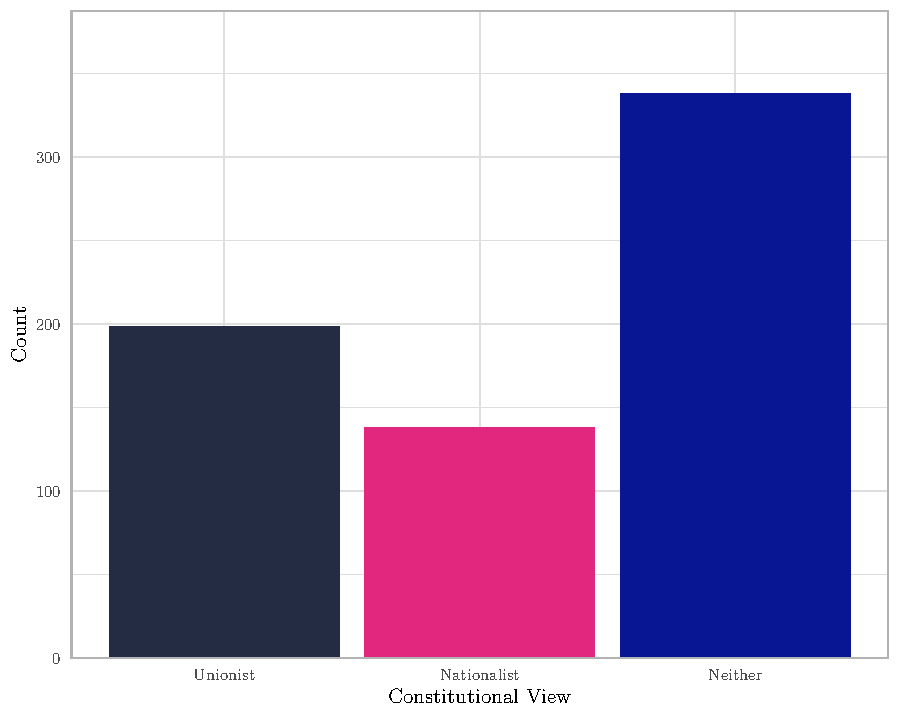
\includegraphics[width=0.8\linewidth]{paper_files/figure-latex/unnamed-chunk-9-1} 

}

\caption{Bar plot of Constitutional View}\label{fig:unnamed-chunk-9}
\end{figure}

\begin{figure}[H]

{\centering 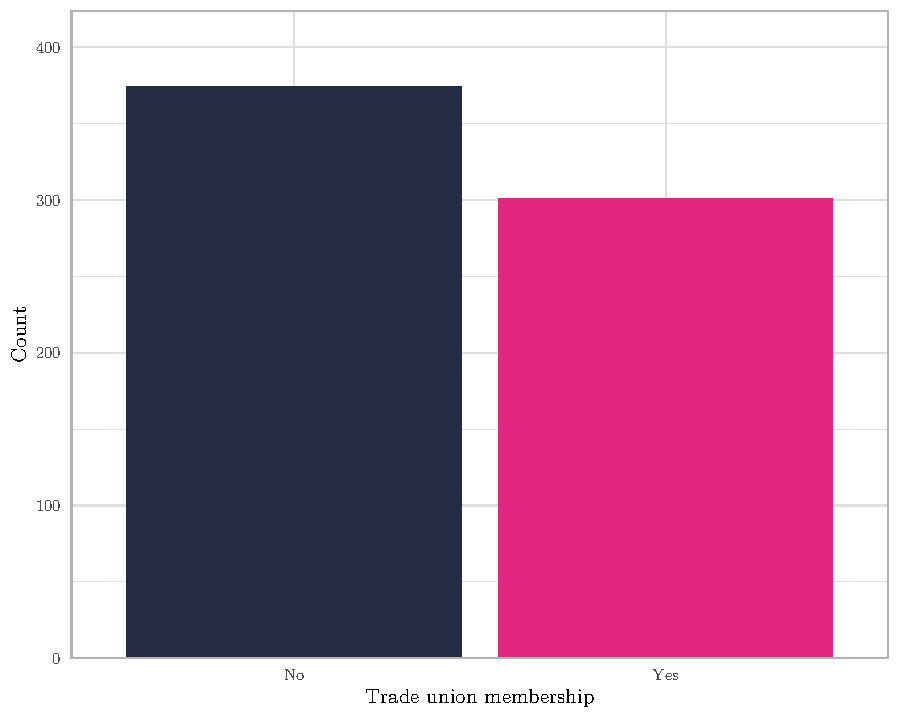
\includegraphics[width=0.8\linewidth]{paper_files/figure-latex/unnamed-chunk-10-1} 

}

\caption{Bar plot of Trade union membership}\label{fig:unnamed-chunk-10}
\end{figure}

\begin{figure}[H]

{\centering 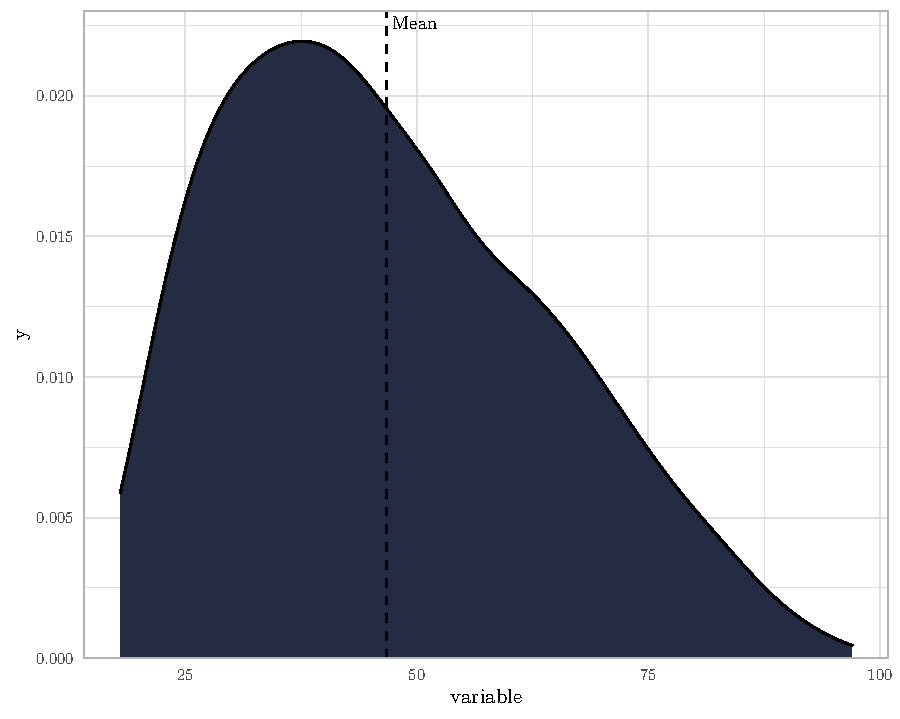
\includegraphics[width=0.8\linewidth]{paper_files/figure-latex/unnamed-chunk-11-1} 

}

\caption{Bar plot of Supervisor}\label{fig:unnamed-chunk-11}
\end{figure}

\begin{figure}[H]

{\centering 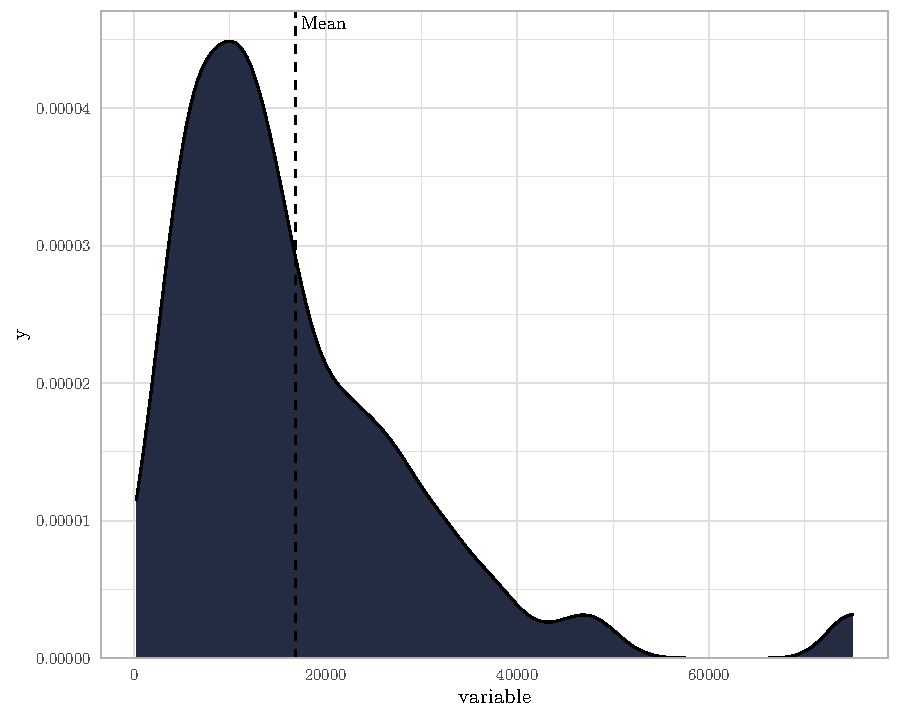
\includegraphics[width=0.8\linewidth]{paper_files/figure-latex/unnamed-chunk-12-1} 

}

\caption{Density plot of Age}\label{fig:unnamed-chunk-12}
\end{figure}

\begin{figure}[H]

{\centering 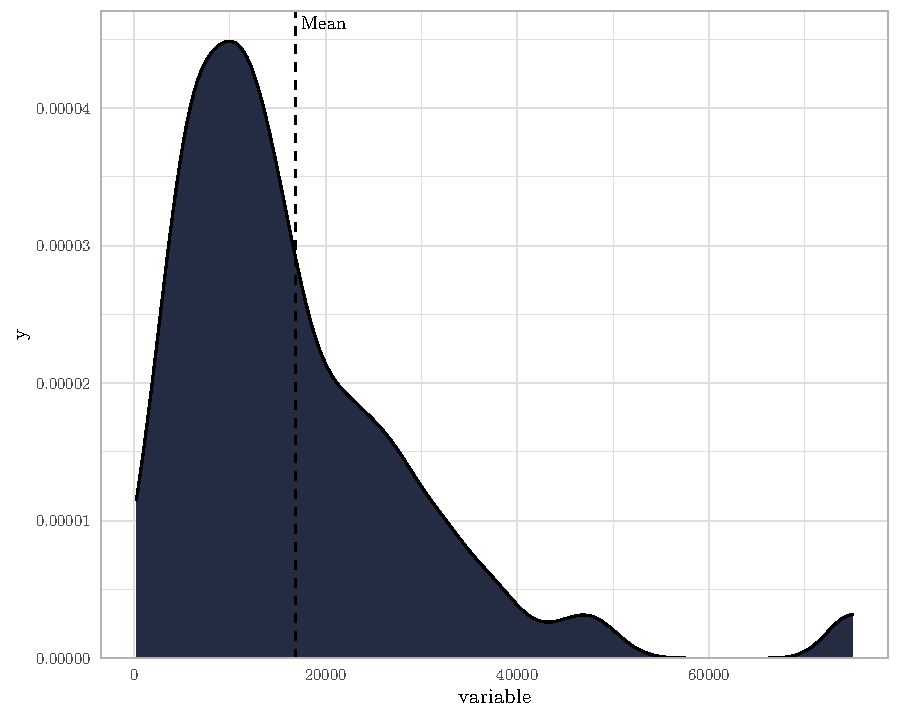
\includegraphics[width=0.8\linewidth]{paper_files/figure-latex/unnamed-chunk-13-1} 

}

\caption{Density plot of Income}\label{fig:unnamed-chunk-13}
\end{figure}

\end{document}
